% mnras_template.tex
%
% LaTeX template for creating an MNRAS paper
%
% v3.0 released 14 May 2015
% (version numbers match those of mnras.cls)
%
% Copyright (C) Royal Astronomical Society 2015
% Authors:
% Keith T. Smith (Royal Astronomical Society)

% Change log
%
% v3.0 May 2015
%    Renamed to match the new package name
%    Version number matches mnras.cls
%    A few minor tweaks to wording
% v1.0 September 2013
%    Beta testing only - never publicly released
%    First version: a simple (ish) template for creating an MNRAS paper

%%%%%%%%%%%%%%%%%%%%%%%%%%%%%%%%%%%%%%%%%%%%%%%%%%
% Basic setup. Most papers should leave these options alone.
\documentclass[a4paper,fleqn,usenatbib]{mnras}

% MNRAS is set in Times font. If you don't have this installed (most LaTeX
% installations will be fine) or prefer the old Computer Modern fonts, comment
% out the following line
\usepackage{newtxtext,newtxmath}
% Depending on your LaTeX fonts installation, you might get better results with one of these:
%\usepackage{mathptmx}
%\usepackage{txfonts}

% Use vector fonts, so it zooms properly in on-screen viewing software
% Don't change these lines unless you know what you are doing
\usepackage[T1]{fontenc}
\usepackage{ae,aecompl}


%%%%% AUTHORS - PLACE YOUR OWN PACKAGES HERE %%%%%

% Only include extra packages if you really need them. Common packages are:
\usepackage{graphicx}	% Including figure files
\usepackage{amsmath}	% Advanced maths commands
\usepackage{amssymb}	% Extra maths symbols
\usepackage{subfig}
\usepackage{enumitem}
%%%%%%%%%%%%%%%%%%%%%%%%%%%%%%%%%%%%%%%%%%%%%%%%%%

%%%%% AUTHORS - PLACE YOUR OWN COMMANDS HERE %%%%%

% Please keep new commands to a minimum, and use \newcommand not \def to avoid
% overwriting existing commands. Example:
%\newcommand{\pcm}{\,cm$^{-2}$}	% per cm-squared

%%%%%%%%%%%%%%%%%%%%%%%%%%%%%%%%%%%%%%%%%%%%%%%%%%

%%%%%%%%%%%%%%%%%%% TITLE PAGE %%%%%%%%%%%%%%%%%%%

% Title of the paper, and the short title which is used in the headers.
% Keep the title short and informative.
\title[Sparse component separation]{Sparse component separation of diffuse thermal dust emission from the Cosmic Infrared Background}

% The list of authors, and the short list which is used in the headers.
% If you need two or more lines of authors, add an extra line using \newauthor
\author[M. O. Irfan et al.]{
Melis O. Irfan,$^{1}$\thanks{E-mail: melis.irfan@cea.fr}
J\'er\^ome Bobin,$^{1}$
Jean-Luc Starck.$^{1}$
%Third Author$^{2,3}$
\\
% List of institutions
$^{1}$Laboratoire CosmoStat, AIM, UMR CEA-CNRS-Paris 7 Irfu, SAp/SEDI, Service d'Astrophysique, \\ CEA Saclay, F-91191 GIF-SUR-YVETTE CEDEX, France.\\
}

% These dates will be filled out by the publisher
\date{Accepted XXX. Received YYY; in original form ZZZ}

% Enter the current year, for the copyright statements etc.
\pubyear{2017}

% Don't change these lines
\begin{document}
\label{firstpage}
\pagerange{\pageref{firstpage}--\pageref{lastpage}}
\maketitle

% Abstract of the paper
\begin{abstract}
Component separation for the {\it{Planck}} HFI data is primarily concerned with thermal dust emission and the cosmic infrared background (CIB). Current separation methods make use of smoothing, through convolution with a Gaussian beam, to decouple thermal dust emission from CIB anisotropies at small angular scales. In this paper we present a new component separation method, {\texttt{premise}}: Parameter Recovery Exploiting Model Informed Sparse Estimates. This method exploits the sparse nature of thermal dust emission for denoising purposes and makes use of informed, initial parameter estimates to calculate all-sky maps of thermal dust temperature and spectral index. The data used are simulation data so as to validate {\texttt{premise}}. We find the percentage difference between the {\texttt{premise}} results and the true values to be 2.9, 5.8, 10.7, 7.4, 5.7 and 6.0 per cent at the 1$\sigma$ level across the full sky for thermal dust temperature, spectral index and intensity at 353, 545, 857 and 3000\,GHz, respectively. Comparison between {\texttt{premise}} and a GNILC-like method over select regions of the sky reveal {\texttt{premise}} to outperform within poor signal to noise areas. 
\end{abstract}

% Select between one and six entries from the list of approved keywords.
% Don't make up new ones.
\begin{keywords}
Cosmology: diffuse radiation, ISM: dust, extinction, Methods: Data Analysis, Methods: Statistical
\end{keywords}

%%%%%%%%%%%%%%%%%%%%%%%%%%%%%%%%%%%%%%%%%%%%%%%%%%

%%%%%%%%%%%%%%%%% BODY OF PAPER %%%%%%%%%%%%%%%%%%

\section{Introduction}

Within our Galaxy dust grains, such as carbonaceous and amorphous silicates \citep{draine}, are heated by inter-stellar, UV radiation. The resulting emission, known as thermal dust emission, is the dominant diffuse Galactic emission at frequencies{\mbox{ $>$ 100\,GHz}} \citep{bennett}. Measurements of thermal dust emission reveal the chemistry of the interstellar medium (\citet{comp11}; \cite{jones}), trace interstellar radiation and reveal dust mass and dust column density. Additionally, thermal dust emission is a prominent astrophysical foreground present in measurements of the cosmic microwave background (CMB). In order to infer cosmological information from measurements of the CMB over 100\,GHz, accurate subtraction of thermal dust emission is crucial \citep{planckCompSep}.

Over large angular-scales thermal dust emission can be modelled as blackbody emission, as can the cosmic infrared background (CIB); diffuse infrared emission from dusty galaxies across all redshifts. The CIB is a strong tracer of the star formation history of the Universe \citep{lagache} and its anisotropies shed light on galaxy clustering and dark matter halo distributions \citep{bethermin}. The similarity in spectral shape between thermal dust emission and the CIB adds complexity to their separation. The correlation between thermal dust and $\rm{H_{I}}$ emission can be used to differentiate between thermal dust and the CIB at large angular scales \citep{pr2} but unfortunately this correlation cannot be exploited at scales smaller than several degrees. 

Since the second {\it{Planck}} data release specific attempts to separate thermal dust emission from the CIB over {\it{Planck}} HFI frequencies have been implemented with increasing success. \citet{pr2} fit a modified blackbody (MBB) to the data and present all-sky maps of the three fit parameters: dust temperature, spectral index and and thermal dust opacity at 353\,GHz. The MBB parameters do not represent the mass-weighted averages of the physical dust properties along the line-of-sight, e.g. the MBB dust temperature is the not the mass-weighted temperature of all the dust particles contributing to the measured emission. Rather, the MBB parameters are simply the empirical parameters which best fit the overall dust emission. This approach is well-suited for component separation, however for an improved understanding of the thermal dust emission mechanism itself more complex models are required (e.g. \citet{draine}; \citet{comp11}; \citet{jones}).

\citet{pr2} introduce a two-stage approach to the customary pixel-by-pixel fit. First they smooth the $N_{\rm{side}}$ 2048 HFI maps to 30 arcmin and fit a MBB with three free parameters to obtain the spectral indices per pixel. Next they fit the 5 arcmin (essentially full resolution) HFI maps, fixing the spectral index values to those obtained at 30 arcmin and allowing two free parameters for the fit. The result being all-sky maps of dust temperature and 353\,GHz opacity at 5 arcmin and spectral index at 30 arcmin. Smoothing the data averages out the CIB anisotropies to a greater extent than it averages out the spatial correlations of thermal dust emission; the CIB has a flatter angular power spectrum than thermal dust. However the effects of smoothing on thermal dust emission are not negligible; \citet{pr2} note the trade-off between sensitivity to small-scale variations of thermal dust emission and smoothing for component separation purposes. The all-sky maps of thermal dust emission formed from the three fitted parameters display variations of 30 per cent, at all scales, from the Finkbeiner, Davis and Schlegel thermal dust model \citep{fds}. 

\citet{gnilc} present an improvement on the \citet{pr2} method by only smoothing the data within the regions where the CIB anisotropies start to dominate the total signal at small angular scales. Their analysis is performed within the needlet (spherical wavelet) domain, where emissions are modelled as transient waveforms within pixel and harmonic space. \citet{gnilc} account for the `nuisance'  (non-thermal dust) contributions using a covariance matrix formed from noise, CIB and CMB estimates. This nuisance covariance matrix is used to identify regions of the sky where thermal dust emission dominates over CIB, CMB and noise, within these regions the separation of thermal dust and CIB is expressed as a convex linear optimisation problem as solved accordingly. Within the nuisance dominated regions the data are smoothed and reassessed, if the nuisance term continues to dominate the width of the Gaussian kernel used for smoothing is increased by a factor of two and the process repeated. Therefore the \citet{gnilc} all-sky estimates of thermal dust emission have a range of effective beam sizes from FWHM = 5.0 arcmin, within the high signal to noise regions (over 65 per cent of the sky) to FWHM = 21.8 arcmin at high Galactic latitudes. The \citet{gnilc} thermal dust maps are shown to be an improvement on the \citet{pr2} maps when the residual CIB maps from both methods and the reduced $\chi^2$ from the MBB fits are compared. The GNILC code however is incredibly computationally intensive as it performs the MBB fit on each pixel for the full resolution {\it{Planck}} data (over fifty million pixels). 

We present a component separation method which builds on the nuisance covariance matrix used in GNILC but introduces sparsity and informed parameter estimates. This method is referred to as {\texttt{premise}}: Parameter Recovery Exploiting Model Informed Sparse Estimates. Within the wavelet domain thermal dust emission can be fully represented using a sparse amount of wavelet coefficients. This is due to the highly correlated nature of thermal dust emission across the sky at each frequency. Conversely, the CIB and instrumental noise can both be approximated as Gaussian noise due to their lack of {\it{strong}} spatial correlations; instrumental noise is faintly correlated across the sky in that it follows the instrument's scanning strategy and the CIB anisotropies are also faintly spatially correlated as they trace galaxy clustering. {\texttt{premise}} uses the covariance matrix aspect of GNILC to filter the contaminated dust maps. However, instead of a completing a pixel-by-pixel MBB fit to the filtered dust maps {\texttt{premise}} divides the full sky into patches treating each patch like a "superpixel" to provide an initial estimate of the full sky temperatures and spectral indices. Each patch size is dependant on the dust properties within said patch. Finding the optimum temperatures and spectral indices per pixel can be achieved using the least squares estimator on the residual between the model maps and the empirical data (thermal dust plus nuisance terms) within the wavelet domain and adding a penalisation factor to favour sparsity, i.e. the fewest number of non-zero wavelet coefficients.

Starting with simulation data representing the combination of thermal dust emission, point sources, instrumental noise, CMB and CIB we apply {\texttt{premise}} to produce estimates of thermal dust emission. The simulated thermal dust emission was created using a single MBB with three parameters: temperature, spectral index and optical depth at 353\,GHz. Fitting the same model to the {\texttt{premise}} thermal dust emission maps provides a comparison between the fitted and the true parameters which can be used to evaluate {\texttt{premise}}. Additionally, we implement a GNIC methodology \citep{gnilc} to enable comparisons between GNILC and {\texttt{premise}}.

The paper is organised as follows: section \ref{sec:data} introduces the simulation data alongside the ancillary data used and the regions of the sky investigated, section \ref{sec:method} details the steps within {\texttt{premise}} and section \ref{sec:results} presents our results in comparison with results obtained via the GNILC methodology.  

\section{Data}
\label{sec:data}
\subsection{Simulated Thermal Dust}

The data used in this paper are simulation data, formed from equation~(\ref{eq:bbinten}).
The GNILC \footnotemark  all-sky temperature and spectral index maps provide the required temperature ($T$)
 and spectral index ($\beta$), the {\it{Planck}} FFP8 \citep{ffp} thermal dust map at 353\,GHz provides the normalisation factor and B denotes the blackbody function.  
\footnotetext{http://pla.esac.esa.int/pla/}
\begin{equation}
S_{\rm{dust}}(\nu) = S_{\rm{ffp8}}(353 \, \rm{GHz}) \times \frac{B(T, \beta, \nu)}{B(T, \beta, 353 \, \rm{GHz})} \times
    \left(\frac{\nu}{353 \, \rm{GHz}}\right)^{\beta} \times \rm{cc}^{-1}.
\label{eq:bbinten}
\end{equation}
The single spectral index model was preferred over the two-index model \citep{meis} as the two-index model has been shown to improve the fit to the data when frequencies below 353\,GHz are used. Equation~(\ref{eq:bbinten}) was evaluated at frequencies 353, 545, 857 and 3000\,GHz to emulate {\it{Planck}} HFI data used in combination with the 100\,$\mu$m IRIS map \citep{iris}. These fluxes were multiplied by their inverse colour corrections ($\rm{cc}^{-1}$) to further align them with real data. The colour corrections were calculated across the {\it{Planck}} HFI bandpasses for frequencies 353, 545 and 857\,GHz. The 3000\,GHz colour correction factors were taken from Table 3 of \citet{iris}. 

Simulation data were not created for the lowest two HFI frequencies (100 and 217\,GHz) following the method of \citep{gnilc}, which fits a modified blackbody (MBB) model to the GNILC 353, 545, 857 and 3000\,GHz maps. The 353\,GHz FFP8 data were neither smoothed nor downgraded, so all our simulation data are at $\rm{N_{side}}$ 2048 with a FWHM of 4.92 arcmin. 

\subsection{Simulated CIB, CMB, noise and point sources}

The simulated total flux maps used differ for the GNILC methodology and {\texttt{premise}}. While GNILC includes the CMB within its covariance matrix of nuisance terms (non-thermal dust contributions to the total flux), {\texttt{premise}} is intended for use on CMB subtracted maps. The total flux maps used for the GNILC methodology were constructed as: 
\begin{equation}
S_{\rm{GNILC}}(\nu) = S_{d}(\nu)  + S_{\rm{CIB}} (\nu) + S_{\rm{CMB}}(\nu)  +  S_{n}(\nu)  + S_{ps}(\nu),
\label{eq:gnilcTotS}
\end{equation}
where $S_{d}(\nu)$ is the thermal dust contribution at each frequency ($\nu$) and $S_{n/ps/\rm{CMB}}(\nu)$ is the FFP8 simulated instrumental noise/point sources/CMB contribution. A 3000\,GHz CIB map of $\rm{N_{side}}$ 2048 and FWHM 5 arcmin was created using the methodology detailed in Appendix C of \citet{pr2}. Gaussian noise with a median level of 0.06 MJy $\rm{sr}^{-1}$ \citep{pr2} was used for the 3000\,GHz noise map. No CMB nor point source contributions were included at 3000\,GHz.  

The total flux maps used for {\texttt{premise}} were constructed as: 
\begin{equation}
S_{\rm{{\texttt{premise}}}}(\nu) = S_{d}(\nu)  + S_{\rm{\widetilde{CIB}}} (\nu) +  S_{\tilde{n}}(\nu)  + S_{ps}(\nu), 
\label{eq:waveTotS}
\end{equation}
where $S_{\rm{\widetilde{CIB}}} (\nu) $ and $S_{\tilde{n}}(\nu) $ are simulated CIB and instrumental noise maps featuring fractional CMB emission, representative of the CIB and noise properties of an intensity map after an imperfect CMB subtraction.  \textcolor{red}{Talk to Jerome for more detail}...

\subsection{LAB data}

Section \ref{cibcontrib} discusses the removal of the large-scale CIB offset through the use of LAB $\rm{H_{I}}$ Survey data. These data are available in the form of all-sky {\texttt{HEALPix}} maps \citep{healpix} at $\rm{N_{side}}$ 512 and a FWHM of \mbox{$\sim$ 36 arcmin}. \footnotemark
\footnotetext{https://lambda.gsfc.nasa.gov}

\subsection{Regions}

We compute {\texttt{premise}} on the full sky, however as GNILC is a computationally intensive algorithm we only run the GNILC methodology on four test regions and conduct our comparison of methods within these four regions, each 256X256 pixels. The regions comprise of a high signal to noise region in the Galactic plane (region 1), a low signal to noise region at intermediate latitude (region 2), a fair signal to noise region at intermediate latitude (region 3) and a low signal to noise polar region (region 4). The location of these regions within a {\texttt{HEALPix}} sphere is shown in Fig.~\ref{fig:globe}. 

\begin{figure}
\centering
\includegraphics[width=0.99\linewidth]{patchesOnGlobe}
\caption{The location on the sphere of the four 256X256 pixel regions chosen for analysis.}
\label{fig:globe}
\end{figure}

\section{Method}
\label{sec:method}
\subsection{Point sources} \label{scontrib}

Point sources were removed from the 353, 545 and 857\,GHz data using the appropriate FFP8 masks for each frequency. The {\texttt{premise}} algorithm is capable of processing masked data as the use of the discrete wavelet transform allows for the reconstruction of the full wavelet, providing the Shannon sampling condition is fulfilled. The GNILC methodology, however, requires each data pixel to provide astrophysical information. Therefore the masked GNILC data were inpainted using a morphological component analysis technique \citep{inpaint}. The total intensity at frequency $\nu$ for pixel $p$ can be considered as follows: 
\begin{equation}
x_{\nu}(p) = a_{\nu} s_{\nu}(p) + z_{\nu}(p),
\label{eq:basic}
\end{equation}
where $z$ represents the Gaussian-like components, CIB and instrumental noise and $a$ is the amplitude of the only emission source ($s$) considered in this work: thermal dust emission. We can simultaneously consider all frequencies and pixels using matrix notation: 
\begin{equation}
{\bf{X}} =  {\bf{A}} {\bf{S}} + {\bf{Z}},
\label{eq:basicmat}
\end{equation}
where the matrix dimensions are the number of the frequency channels by the number of pixels. The contribution of the masked pixel to the reconstruction of the full wavelet is nullified within the least squares optimisation as follows: 
\begin{equation}
\min_{A, S} \, \frac{1}{2} \| M \times ({\bf{X}} - {\bf{AS}})  \|^{2} + \Lambda \| {\bf{S}}  \Phi^{T}  \|, 
\end{equation}   
where $M$ is the mask to be applied to the data with pixels of magnitude 1 or 0 and the last term represents a penalisation factor favouring sparse solutions in the wavelet domain.   

\subsection{CIB, CMB and noise contributions} \label{cibcontrib}

We implement two algorithms: our own, {\texttt{premise}} and a GNILC-like methodology. The principal steps for both algorithms are summarised in Fig.~\ref{fig:methFlo}: removing large-scale CIB offsets, filtering small-scale anisotropies and fitting a MBB. 

\begin{figure}
\centering
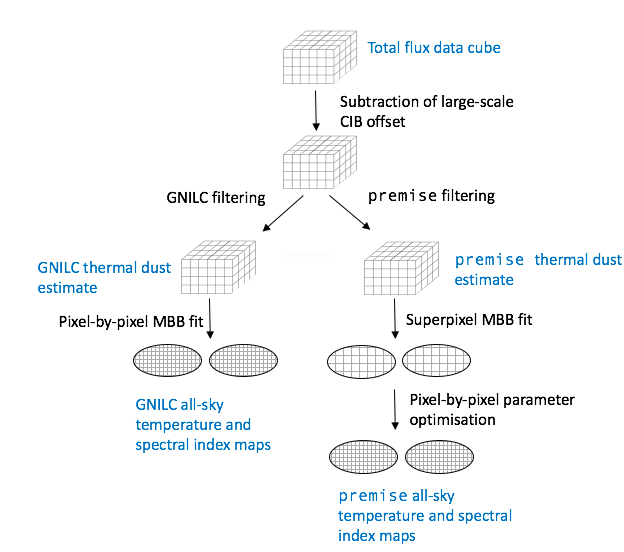
\includegraphics[width=0.99\linewidth]{methodDiagram}
\caption{The principal steps of the both the GNILC and {\texttt{premise}} algorithms.}
\label{fig:methFlo}
\end{figure}

The CIB is seen to contribute to the overall measured intensity in two ways: small-scale variations and a large-scale intensity which manifest as a constant, additive offset to the pure thermal dust intensity. Fig.~\ref{fig:ciboffset} shows a 1D slice of region 3 at 353\,GHz. The green line shows the total emission while the blue line shows the pure thermal dust emission. The large-scale CIB contribution can clearly be seen as a positive offset while the small-scale CIB contributions, alongside instrumental noise, are seen as Gaussian-like variations around the thermal dust mean level. 

\begin{figure}
\centering
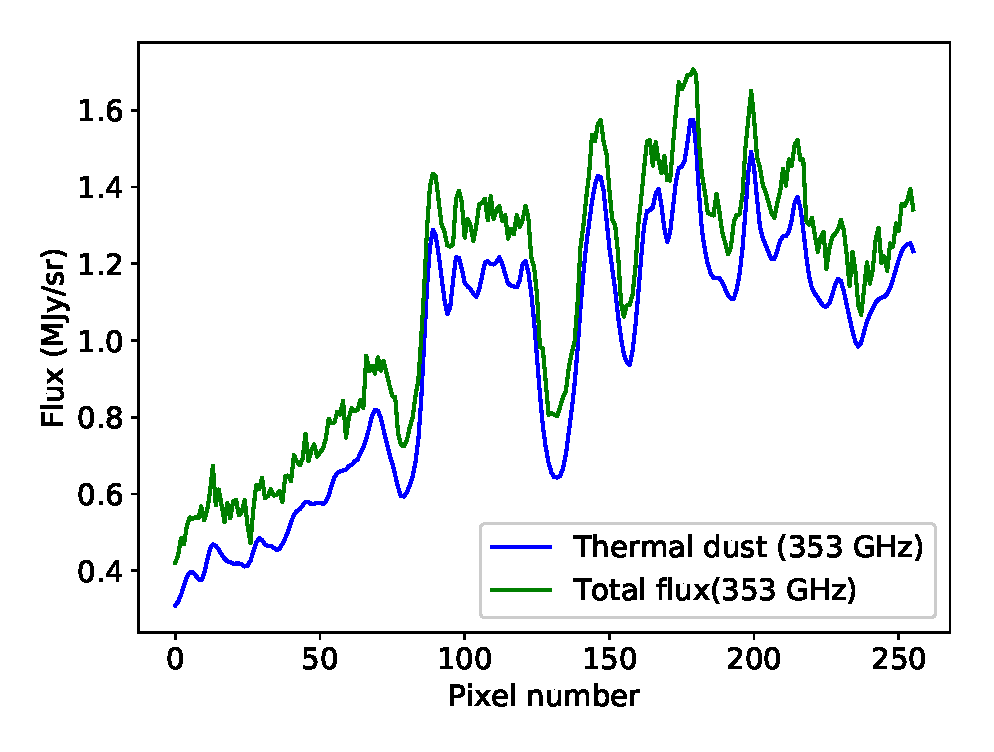
\includegraphics[width=0.8\linewidth]{ciboffset353face6}
\caption{One dimensional slice of region 3 at 353\,GHz. The green line represents thermal dust + CIB + instrumental noise, the blue line is just thermal dust.}
\label{fig:ciboffset}
\end{figure}

\subsubsection{Large angular scales}

The first step of {\texttt{premise}} is to remove the large-scale CIB offset. The constant CIB offsets for each frequency were calculated using the method described in \citet{pr2}, see Appenidx \ref{sec:apA} for details. The resulting offsets were found to be 0.126, 0.331, 0.641 and 0.657 MJy $\rm{sr^{-1}}$ for 353, 545, 857 and 3000\,GHz respectively.  These values were subtracted from the total flux maps. The mean values for the simulated CIB maps are 0.140, 0.366, 0.718 and 0.718 MJy\,sr$^{-1}$, placing an 8.5 -- 11 per cent error on the linear regression method.

\subsubsection{Small angular scales}

Both {\texttt{premise}} and GNILC make use of a covariance matrix of the combined `nuisance' terms to locate dimensions within signal subspace where the desired signal, thermal dust emission in this case, is dominant. For {\texttt{premise}} the nuisance terms are the small-scale CIB and instrumental noise whereas for GNILC the nuisance terms are the same plus the CMB. As this paper is concerned with simulation data the exact CIB, CMB and instrumental noise maps used to make the total flux maps are given as nuisance term estimates, therefore the estimation of the nuisance covariance matrix is unrealistically perfect. 

The GNILC methodology we implement is not identical to that described in \citet{gnilc}, therefore we detail our GNILC filtering technique in Appendix \ref{sec:apB}, highlighting any differences. The {\texttt{premise}} filtering, based on the GNILC filtering is as follows: 

\textcolor{red}{Description of filtering code}

\subsection{Fitting the MBB model}

Both the GNILC methodology and {\texttt{premise}} involve a fit to the following MBB model:
\begin{equation}
S_{\rm{dust}}(\nu) = \tau_{353} \times B(T, \beta, \nu) \times \left(\frac{\nu}{353 \, \rm{GHz}}\right)^{\beta} \times \rm{cc}^{-1},
\end{equation}
where the optical depth at 353\,GHz ($\tau_{353}$), the dust temperature ($T$) and the thermal dust spectral index ($\beta$) were the free parameters in the fit. The inverse colour correction ($\rm{cc}^{-1}$) also depends on $T$ and $\beta$. 

\begin{figure}
\centering
\subfloat{\includegraphics[width=0.99\linewidth]{fullskyPatches}}
\caption{All-sky map of the different patches chosen by the quadtree.}
\label{fig:patches}
\end{figure}

For the GNILC methodology the MBB model is simply fit pixel-by-pixel to the GNILC estimate of thermal dust emission. For {\texttt{premise}} the fitting is more complex; it makes use of the quadtree technique. A quadtree recursively divides the given data into quarters until a particular criteria is no longer achieved within the patch of data. The quadtree used in this method recursively divides a square of data until the number of data points (in this case, reduced $\chi^{2}$ values) with a value greater than 2 within the patch are less than 10 per cent of the total number of data points. A lower limit of 8 is enforced to ensure that the quadtree cannot split the data into patches smaller than 8X8 pixels. The quadtree is also prohibited from splitting a patch into quarters if one or more of those quarters contains only masked data. Fig.~\ref{fig:patches} shows the patches selected by the quadtree over the full sky. The patches sizes are visibly smaller within and near to the Galactic plane where the total flux across neighbouring pixels is less consistent than at high latitudes. Very close to the Galactic centre several patch sizes larger than their neighbouring patches can be seen: these areas contain so many masked pixels (due to point sources) that the quadtree is forbidden from dividing the region into smaller areas.  

The {\texttt{premise}} fitting processes works on each of the twelve 2048X2048, {\texttt{HEALPix}} 2D faces which make up the full sky as follows:
\begin{enumerate}[label*=\arabic*.]
\item The noise covariance matrix ($R_{n}$) of the full data face is calculated within the wavelet domain for four wavelet scales ($j$):
\begin{equation}
R_{n}(j) = \frac{1}{2048^2} \left( \Phi_{n}(j) \, {\rm{X}}  \, \Phi_{n}^{T}(j) \right),
\end{equation} 
where $\Phi_{n}$ is the wavelet transform of the instrumental noise plus the CIB anisotropies (large-scale CIB offsets removed). 
\item The region is split into patches of 128X128
\item Each patch is treated as a superpixel: the mean flux density for each frequency represents the whole patch at that frequency	
\item An MBB fit to each superpixel yields the parameters required to form a thermal dust estimate for each frequency at that superpixel ($P$).
\item The data-model residual is calculated per original pixel ($p$):
\begin{equation}
\rm{Residual}($p$) = \rm{Total \, Flux}(p) -  \rm{Estimated \, thermal \, dust \, flux}(P)
\end{equation}
\item This residual matrix (${\rm{N_{obs}}}$ by ${\rm{N_{pix}}}$ ) is transformed into the wavelet domain using four wavelet scales ($\Phi_{r}(j)$). 
\item The reduced $\chi^{2}$ at each of the four wavelet scales ($j$) is calculated for each pixel:
\begin{equation}
\chi^{2}_{\rm{red}}(j, p) = \Phi_{r}(j) \, \left( \Phi_{n}(j)^{-1} \, \Phi_{r}(j) \right)
\end{equation}
As there is only one degree of freedom the reduced $\chi^{2}$ is just the $\chi^{2}$.
\item The reduced $\chi^{2}$ is fed back into the quadtree to split the data into patches where $T$ and $\beta$ are constant enough to be well characterised by a MBB with a single value of $T$ and $\beta$ across all pixels within the patch. The higher wavelet scales are used for larger patch sizes so when deciding whether or not to split a 64X64 patch the quadtree uses the reduced $\chi^{2}$ values from the fourth wavelet scale, for a 16X16 patch the first wavelet scale is used. The final patches chosen are the quadtree determined superpixels.  
\item The fit is re-run fit on the quadtree chosen superpixels and initial maps of $T$ and $\beta$ estimates are obtained.
\end{enumerate}

Running the MBB fit on super-pixels, as opposed to the true pixels, reduces the computational time by, at minimum, a factor of 64 (the minimum patch area being 64 pixels).  

\subsection{Parameter optimisation}

\textcolor{red}{Description of pixel code}.

\section{Results}
\label{sec:results}

\subsection{Comparison of methods within Regions 1--4}

\subsubsection{Thermal dust maps}

Both the GNILC methodology and {\texttt{premise}} remove the large-scale CIB offsets at each frequency and filter the total flux maps to provide estimates of pure thermal dust per observational frequency. Fig.~\ref{fig:percentAll} compares the inpainted \citep{inpaint} {\texttt{premise}} and GNILC all-sky estimates for thermal dust emission for each of the four regions. Note that while inpainting is used to produce {\texttt{premise}} all-sky thermal dust estimates, no inpainting is required to obtained the thermal dust fitted parametrs. Mean percentage difference from the pure thermal dust is shown in the main images while the percentage difference for each frequency (353, 545, 857 and 3000\,GHz) are shown in the insets. The {\texttt{premise}} thermal dust estimates provide the closest representation to the true dust flux values for all four regions specifically outperforming the standard GNLIC filtering at low signal to noise (353\,GHz and region 4).

\begin{figure}
\centering
\subfloat{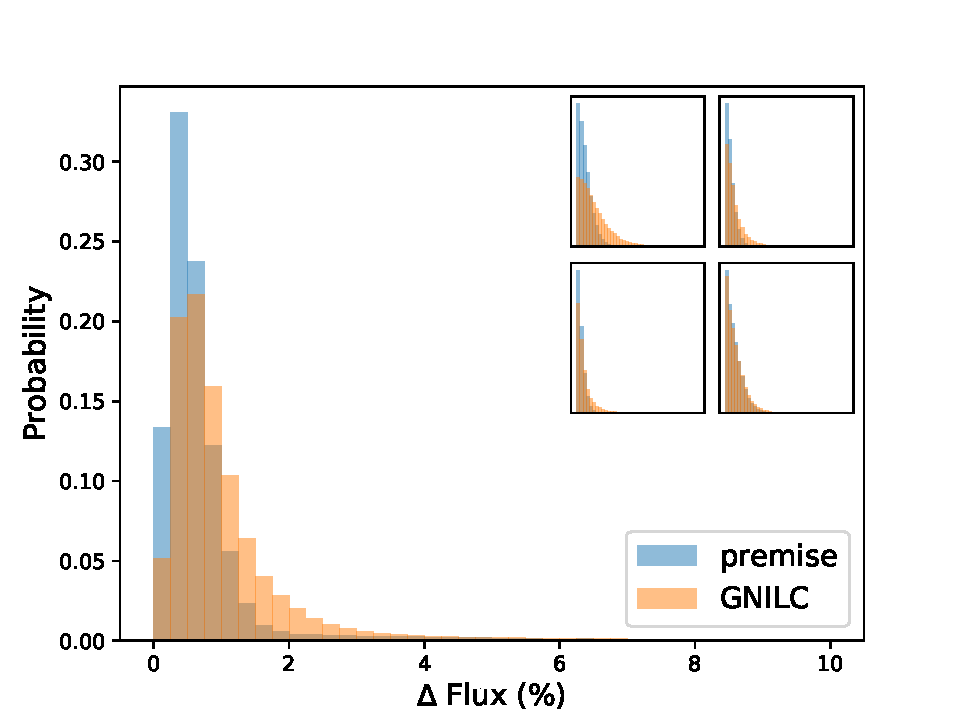
\includegraphics[width=0.85\linewidth]{dustdiff1}}\,
\subfloat{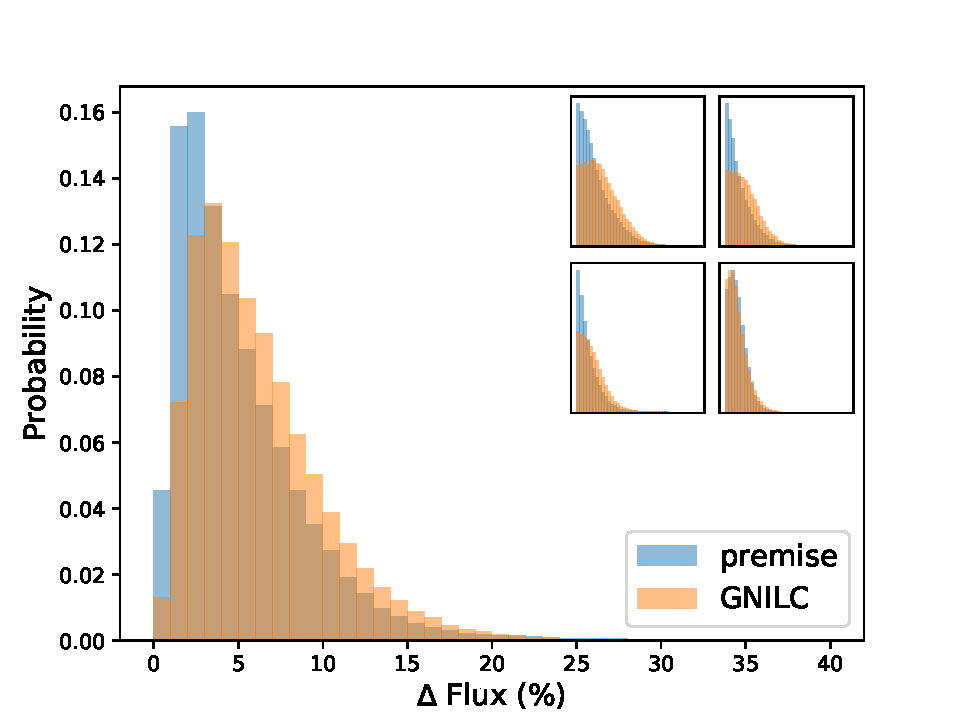
\includegraphics[width=0.85\linewidth]{dustdiff5}}\,
\subfloat{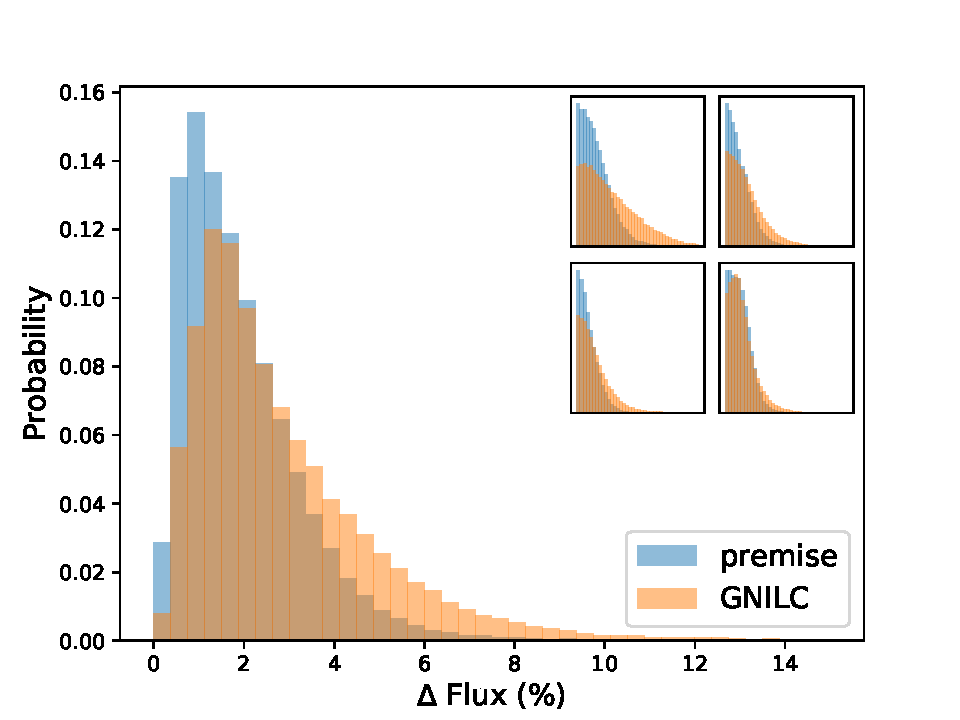
\includegraphics[width=0.85\linewidth]{dustdiff6}}\,
\subfloat{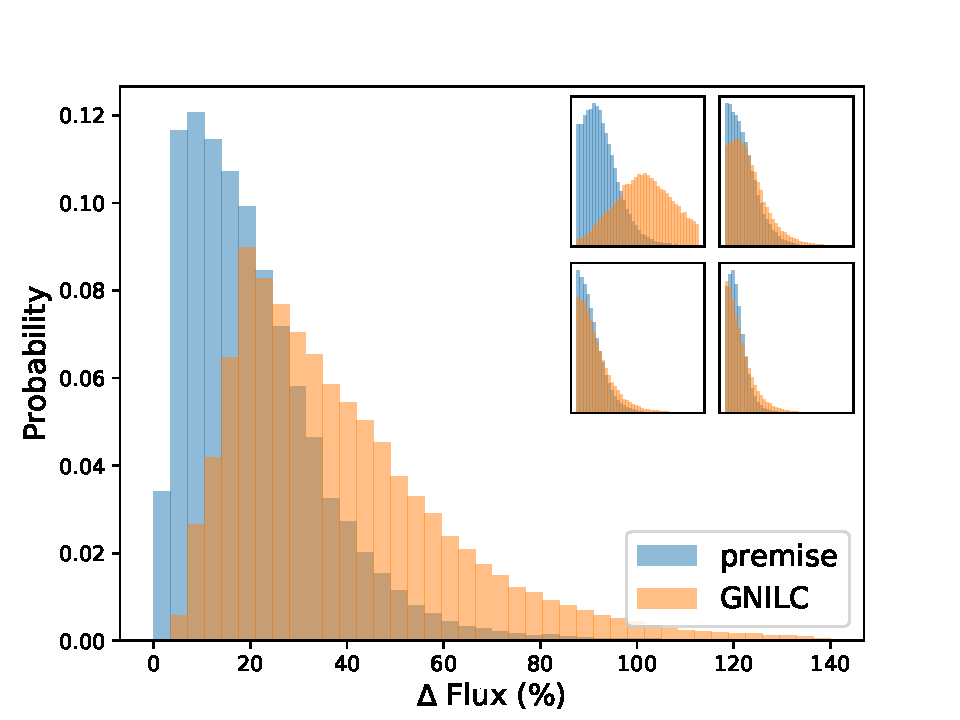
\includegraphics[width=0.85\linewidth]{dustdiff9}}\,
\caption{Mean percentage difference across all four frequencies between pure thermal dust emission and the GNILC/{\texttt{premise}} dust estimate for region 1, 2, 3 and 4 ({\it{top to bottom}}). Insets show the percentage difference for each frequency 353 ({\it{top left}}), 545 ({\it{top right}}), 857 ({\it{bottom left}}) and 3000\,GHz ({\it{bottom right}}).}
\label{fig:percentAll}
\end{figure}

The reduced $\chi^{2}$ for the {\texttt{premise}} dust maps can be calculated as: 
\begin{equation}
\chi^{2}_{\rm{red}} = \frac{1}{d.o.f.} {\bf{(E - X)}} {\bf{R}}_{n}^{-1} {\bf{(E - X)}}, 
\end{equation} 
where there are four degrees of freedom ($d.o.f$), $E$ is the $\rm{N_{obs}}$ by $\rm{N_{pix}}$ matrix of expected dust intensities (the simulated pure thermal dust maps), ${\bf{R}}_{n}$ is the $\rm{N_{obs}}$ by $\rm{N_{obs}}$ matrix of "noise" terms: CIB - large-scale constant offset + instrumental noise and $X$ is the $\rm{N_{obs}}$ by $\rm{N_{pix}}$ matrix of estimated thermal dust maps. 

The reduced $\chi^{2}$ values were calculated both in the pixel domain and in the wavelet domain (i.e the expected, empirical and noise maps were wavelet transformed). The wavelet $\chi^{2}$ values are shown for the first wavelet scale. The wavelet transformation removes the effect of large scale variations from the calculation of the $\chi^{2}$ values; for instance the addition of a constant offset to the either the empirical of expected maps would have no effect on the $\chi^{2}$ within the wavelet domain. What is highlighted in the wavelet domain are any localised (on the scale of the data) variations between the empirical and the expected model. The total point sources mask (combination of the 353, 545 and 857\,GHz masks) has been applied to the maps shown in Fig.~\ref{fig:redchi1} -- Fig.~\ref{fig:redchi4}, as the wavelet $\chi^{2}$ is sensitive to the poorer estimation of thermal dust emission associated with inpainting. The lowest $\chi^{2}$ values within the pixel $\chi^{2}$ maps correspond to region 4, the lowest signal to noise region. This is indicative of an underestimation of the noise term as the $\chi^{2}$ values are tracing the noise properties of the data, as opposed to being sensitive to the variations between empirical and expected values. The fact that the wavelet $\chi^{2}$ maps do not identify any poorly fit regions, aside from the inpainted regions, is an additional indicator that it is the noise properties that dominate the information provided by the  $\chi^{2}$ analysis. The noise underestimation stems from faint spatial correlations present within the small-scale CIB anisotropies; a correlated noise covariance matrix cannot be used to accurately whiten the data matrix. 

\begin{figure}
\centering
\includegraphics[width=0.9\linewidth]{redchiFace1wave}
\caption{{\it{(Left to right)}} Reduced $\chi^{2}$ map of region 1 for {\texttt{premise}} in the wavelet domain (first wavelet scale). Reduced $\chi^{2}$ map of region 1 for {\texttt{premise}} in the pixel domain.}
\label{fig:redchi1}
\end{figure}

\begin{figure}
\centering
\includegraphics[width=0.9\linewidth]{redchiFace5wave}
\caption{{\it{(Left to right)}} Reduced $\chi^{2}$ map of region 2 for {\texttt{premise}} in the wavelet domain (first wavelet scale). Reduced $\chi^{2}$ map of region 2 for {\texttt{premise}} in the pixel domain.}
\label{fig:redchi2}
\end{figure}

\begin{figure}
\centering
\includegraphics[width=0.9\linewidth]{redchiFace6wave}
\caption{{\it{(Left to right)}}  Reduced $\chi^{2}$ map of region 3 for {\texttt{premise}} in the wavelet domain (first wavelet scale). Reduced $\chi^{2}$ map of region 3 for {\texttt{premise}}  in the pixel domain.}
\label{fig:redchi3}
\end{figure}

\begin{figure}
\includegraphics[width=0.9\linewidth]{redchiFace9wave}
\caption{{\it{(Left to right)}}  Reduced $\chi^{2}$ map of region 4 for {\texttt{premise}} in the wavelet domain (first wavelet scale). Reduced $\chi^{2}$ map of region 4 for {\texttt{premise}}  in the pixel domain.}
\label{fig:redchi4}
\end{figure}


\subsubsection{Parameter estimation}

In the following section we compare the GNILC and {\texttt{premise}} fitted $T$ and $\beta$ for Regions 1--4 to the true $T$ and $\beta$. Fig.~\ref{fig:histmap1} -- Fig.~\ref{fig:histmap9} show histograms/maps of the actual/percentage differences between the true parameter values and those derived from the GNILC methodology/{\texttt{premise}}. Smaller differences between the true and fitted parameters can be seen for {\texttt{premise}} within regions 2, 3 and 4 but specifically regions 2 and 4, were the thermal dust signal to noise ratio is lowest. For the highest signal to noise region (region 1) {\texttt{premise}} and the GNILC methodology can be seen to produce fairly similar results with {\texttt{premise}} outperforming GNILC for spectral indices and vice-versa for temperature.  

\begin{figure*}
\centering
\subfloat{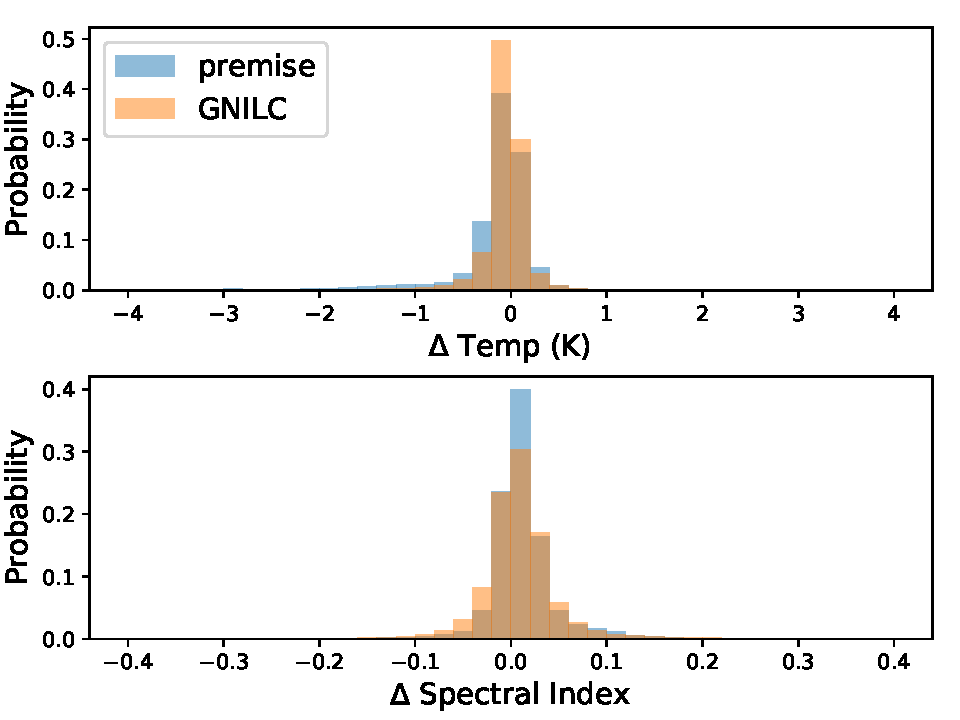
\includegraphics[width=0.4\linewidth]{histFace1}}\,
\subfloat{\includegraphics[width=0.4\linewidth]{mapsFace1}}\,
\caption{Histograms of the differences between model and true temperature/spectral index for the GNILC methodology and {\texttt{premise}} for region 1 ({\it{left}}). Map of percentage differences between model and true temperature/spectral index for the GNILC methodology and {\texttt{premise}} for each pixel in region 1 ({\it{right}}).}
\label{fig:histmap1}
\end{figure*}

\begin{figure*}
\centering
\subfloat{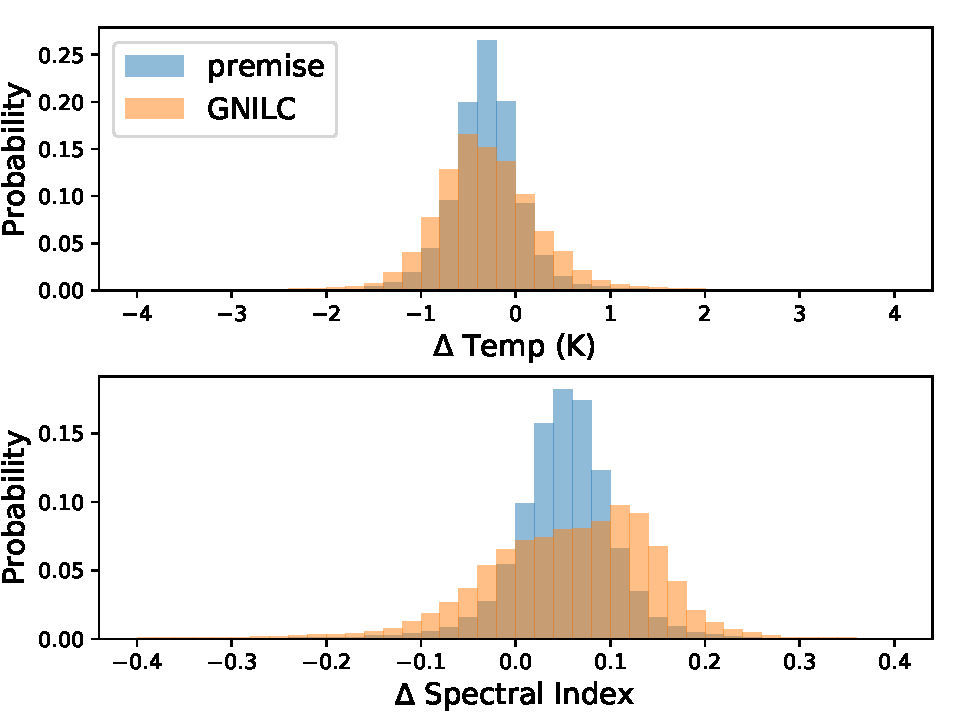
\includegraphics[width=0.4\linewidth]{histFace5}}\,
\subfloat{\includegraphics[width=0.4\linewidth]{mapsFace5}}\,
\caption{Histograms of the differences between model and true temperature/spectral index for the GNILC methodology and {\texttt{premise}} for region 2 ({\it{left}}). Map of percentage differences between model and true temperature/spectral index for the GNILC methodology and {\texttt{premise}} for each pixel in region 2 ({\it{right}}).}
\label{fig:histmap5}
\end{figure*}

\begin{figure*}
\centering
\subfloat{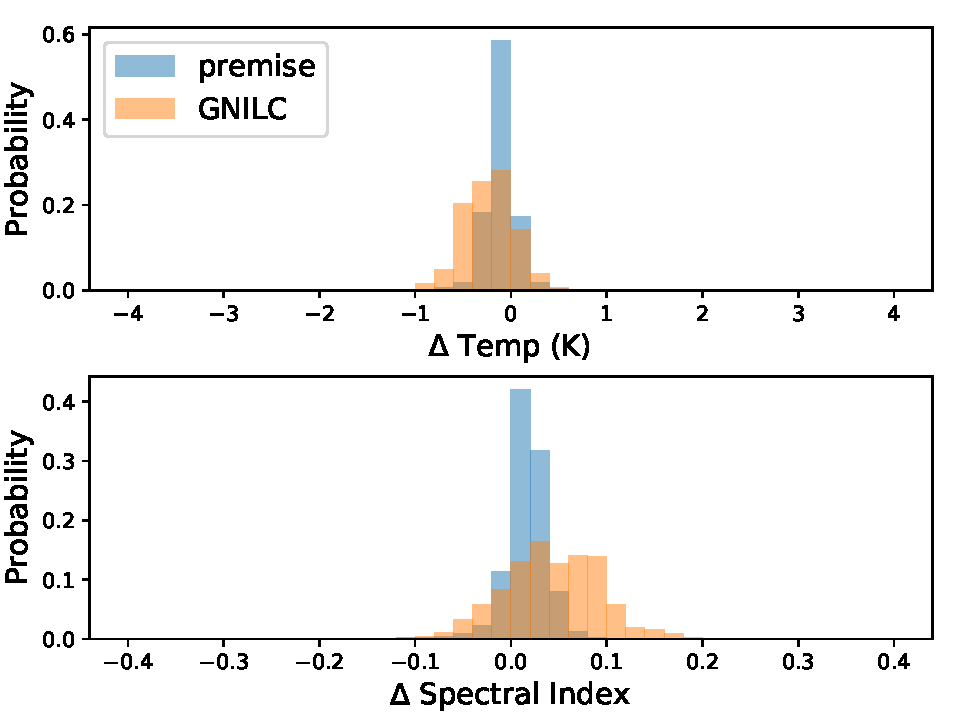
\includegraphics[width=0.4\linewidth]{histFace6}}\,
\subfloat{\includegraphics[width=0.4\linewidth]{mapsFace6}}\,
\caption{Histograms of the differences between model and true temperature/spectral index for the GNILC methodology and {\texttt{premise}} for region 3 ({\it{left}}). Map of percentage differences between model and true temperature/spectral index for the GNILC methodology and {\texttt{premise}} for each pixel in region 3 ({\it{right}}).}
\label{fig:histmap6}
\end{figure*}

\begin{figure*}
\centering
\subfloat{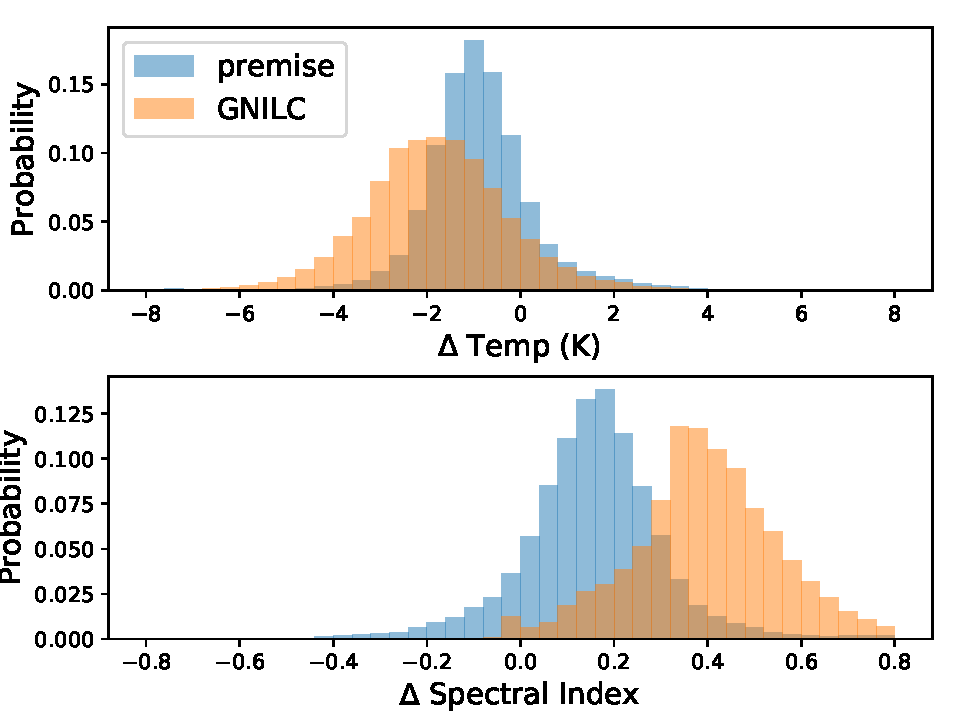
\includegraphics[width=0.4\linewidth]{histFace9}}\,
\subfloat{\includegraphics[width=0.4\linewidth]{mapsFace9}}\,
\caption{Histograms of the differences between model and true temperature/spectral index for the GNILC methodology and {\texttt{premise}} for region 4 ({\it{left}}). Map of percentage differences between model and true temperature/spectral index for the GNILC methodology and {\texttt{premise}} for each pixel in region 4 ({\it{right}}).}
\label{fig:histmap9}
\end{figure*}

\subsection{Full sky {\texttt{premise}}}

\begin{figure*}
\centering
\subfloat{\includegraphics[width=0.5\linewidth]{fullsky353}}
\subfloat{\includegraphics[width=0.5\linewidth]{fullsky545}}\,
\subfloat{\includegraphics[width=0.5\linewidth]{fullsky857}}
\subfloat{\includegraphics[width=0.5\linewidth]{fullsky3000}}\,
\caption{All-sky maps of thermal dust emission produced by {\texttt{premise}} filtering at 353 ({\it{top left}}), 545 ({\it{top right}}), 857 ({\it{bottom left}}) and 3000\,GHz ({\it{bottom right}}). A histogram colour scale has been used.}
\label{fig:dustmaps}
\end{figure*}

\begin{figure*}
\centering
\subfloat{\includegraphics[width=0.5\linewidth]{fullskyTemp}}
\subfloat{\includegraphics[width=0.5\linewidth]{fullskyBeta}}\,
\caption{All-sky maps of thermal dust temperature ({\it{left}}) and spectral index ({\it{right}}) produced by {\texttt{premise}}. Actual temperature range is 10 -- 30 K, actual spectral index range is 1.0 to 2.2.}
\label{fig:paramsmaps}
\end{figure*}

\begin{figure}
\centering
\subfloat{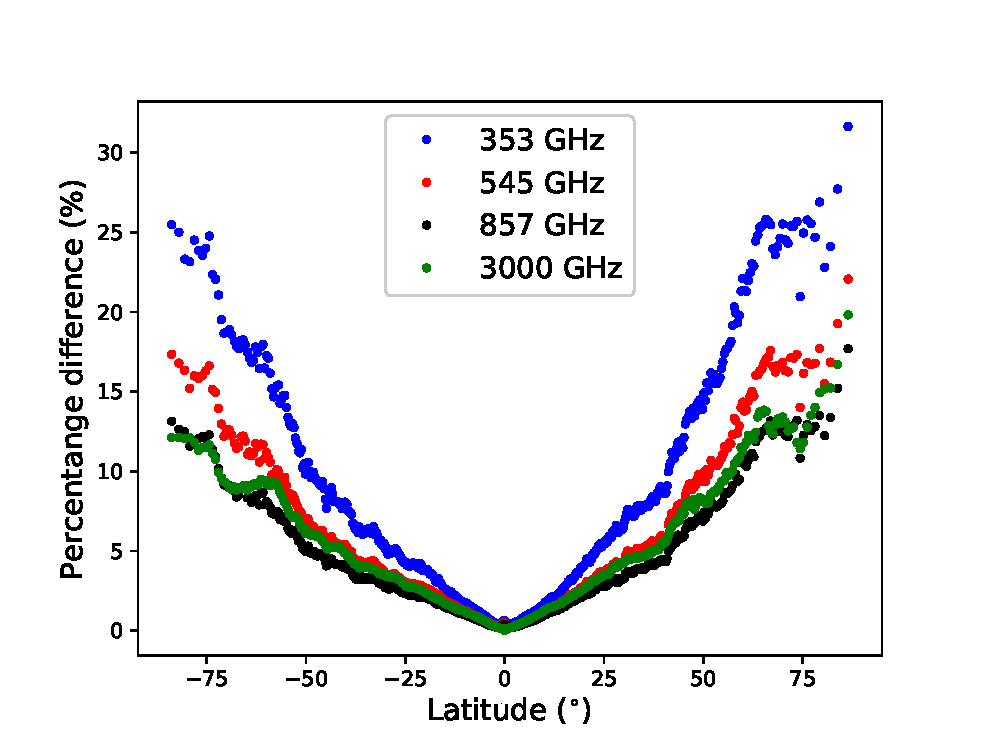
\includegraphics[width=0.85\linewidth]{DustOverLat}}\,
\subfloat{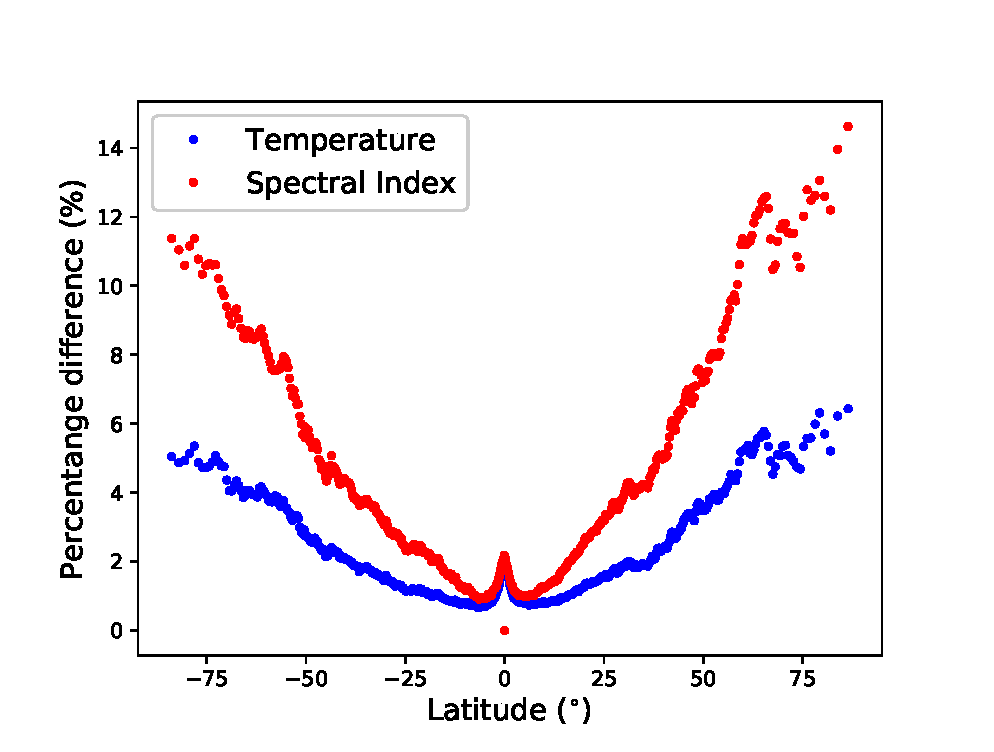
\includegraphics[width=0.85\linewidth]{ParamsOverLat}}\,
\caption{Median percentage difference between true and {\texttt{premise}} estimated thermal dust values as a function of Galactic latitude.}
\label{fig:lats}
\end{figure}

The all-sky {\texttt{premise}} thermal dust temperature, spectral index and emission maps for 353, 545 857 and 3000\,GHz are shown in Fig.~\ref{fig:dustmaps} and Fig.~\ref{fig:paramsmaps}. Table~\ref{tab:accstats} states the percentage difference between true and {\texttt{premise}} estimated thermal dust values for 50 per cent (medium), 68.3 per cent (1$\sigma$), 95.4 per cent (2$\sigma$) and 99.7 per cent (3$\sigma$) of the full sky.

\begin{table}
 \caption{The percentage difference between true and {\texttt{premise}} estimated thermal dust values for various percentiles.}
 \label{tab:accstats}
 \begin{tabular}{l| c| c| c| c}
\hline
{\bf{Value}} &{\bf{ Medium $\% \Delta$}}  & {\bf{1$ \sigma \, \% \Delta$}}  & {\bf{2$ \sigma \, \% \Delta$}}  & {\bf{3$ \sigma \, \% \Delta$}}  \\ 
Temperature & 1.8 & 2.9 & 7.9 & 15.7 \\
Spectral index & 3.5 & 5.8 & 15.2 & 24.6 \\
353\,GHz flux & 5.3 & 10.7 & 44.8 & 116.3 \\
545\,GHz flux & 3.6 & 7.4 & 32.4 & 85.7 \\
857\,GHz flux & 2.9 & 5.7 & 25.6 & 69.3 \\
3000\,GHz flux & 3.4 & 6.0 & 24.8 & 78.9 \\
  \hline
 \end{tabular}
\end{table}

The success of {\texttt{premise}} is proportional to the thermal dust signal to noise ratio; this is highlighted in Fig.~\ref{fig:lats} which shows the medium percentage difference between true and {\texttt{premise}} estimated values across latitudes. Both the thermal dust flux estimates and the parameter estimates decrease in accuracy as distance from the Galactic plane increases. The peak in percentage difference within the Galactic plane (latitude 0$^{\circ}$) is caused by a high fraction of the data being masked due to point sources. 

\section{Conclusions}
We have implemented an improvement on the GNILC method of filtering to produce pure thermal dust maps from simulated total flux maps consisting of CIB, instrumental noise and masked out point sources. When compared to the true maps of simulated pure thermal dust emission, our dust maps have median percentage errors of 5.3, 3.6, 2.9 and 3.4 per cent at 353, 545, 857 and 3000\,GHz, resepctively. We also present a new method of parametric fitting based around informed, initial estimates of parameter values. Full sky data are divided into patches of various size where each patch area contains only those pixels which share similar thermal dust properties. The MBB model (in principal it can be any emission model) is fit to each patch producing an all-sky estimate of model parameters. These parameter estimates are then refined using a sparsity-based optimisation method to produce the final, pixel-by-pixel parameter estimates. In this work we fit for the thermal dust temperature and spectral index and produce all-sky maps of these two values with median percentage errors of 1.8 and 3.5 per cent, resepctively. \textcolor{red}{Need to talk about why we do not fit for tau/normalisation parameter here}. 

By comparing {\texttt{premise}} to a GNILC-like method over select regions of the sky we find that {\texttt{premise}} excels in regions of low signal to noise, producing more accurate temperature and spectral index values than the GNILC-like method in regions out of the Galactic plane. Within the Galactic plane (region 1) {\texttt{premise}} and the GNILC methodology can be seen to produce fairly similar results. The improvement on foreground parameter estimation presented in this work is intended for use in combined foreground estimation algorithms such as \citet{gmca} where other parameters, such as dust or electron temperature, emission measure etc. can be determined by {\texttt{premise}}.
\section*{Acknowledgements}

%%%%%%%%%%%%%%%%%%%%%%%%%%%%%%%%%%%%%%%%%%%%%%%%%%

%%%%%%%%%%%%%%%%%%%% REFERENCES %%%%%%%%%%%%%%%%%%

% The best way to enter references is to use BibTeX:
\bibliographystyle{mnras}
\bibliography{refs} % if your bibtex file is called example.bib


%%%%%%%%%%%%%%%%%%%%%%%%%%%%%%%%%%%%%%%%%%%%%%%%%%

%%%%%%%%%%%%%%%%% APPENDICES %%%%%%%%%%%%%%%%%%%%%

\appendix

\section{Large-scale CIB offset}\label{sec:apA}

To determine the large-scale CIB offset for each frequency data from the Leiden/Argentine/Bonn (LAB) $\rm{H_{I}}$ survey \citep{lab} were used. The LAB data are integrated over radial velocity and three maps are available: the low velocity map (-30 to 30 km $\rm{s}^{-1}$), the intermediate velocity map (-100 to -30 km $\rm{s}^{-1}$) and the high velocity map (-500 to -100 km $\rm{s}^{-1}$). 

The total flux and the LAB low and intermediate velocity all-sky maps were downgraded to $\rm{N_{side}}$ 128 and smoothed to $1^{\circ}$. Two masks were then made which selected pixels for use depending on their column densities ($N_{\rm{H_{I}}}$) within the low and intermediate velocity maps :

\begin{tabular}{ l | c | c  }
\hline
  Mask & Low $N_{\rm{H_{I}}}$ ($\rm{cm}^{-2}$) & Intermediate $N_{\rm{H_{I}}}$ ($\rm{cm}^{-2}$)  \\
  \hline
  1 &  $< 2 \times 10^{20}$  & $ < 0.1 \times 10^{20}$ \\
  2 &  $ < 3 \times 10^{20}$  & -- \\
  \hline
\end{tabular}

Linear regression was used to determine the large-scale CIB offsets using the following pixels and binning: 

\begin{tabular}{ l | c | c  }
\hline
 x axis data & y axis data & Mask applied \\
  \hline
  3000\,GHz & low + intermediate LAB & 2 \\ 
  857\,GHz &  low + intermediate LAB & 1 \\
  545\,GHz & 857\,GHz - offset & 1 \\
  353\,GHz & 857\,GHz - offset & 1 \\
  \hline
\end{tabular}

Fig.~\ref{fig:ciboffsetLinear} shows the linear regression between the 545\,GHz and the 857\,GHz total flux binned, mask 1 pixels. The 857\,GHz offset has been removed from the 857\,GHz data for the linear regression. 

\begin{figure}
\centering
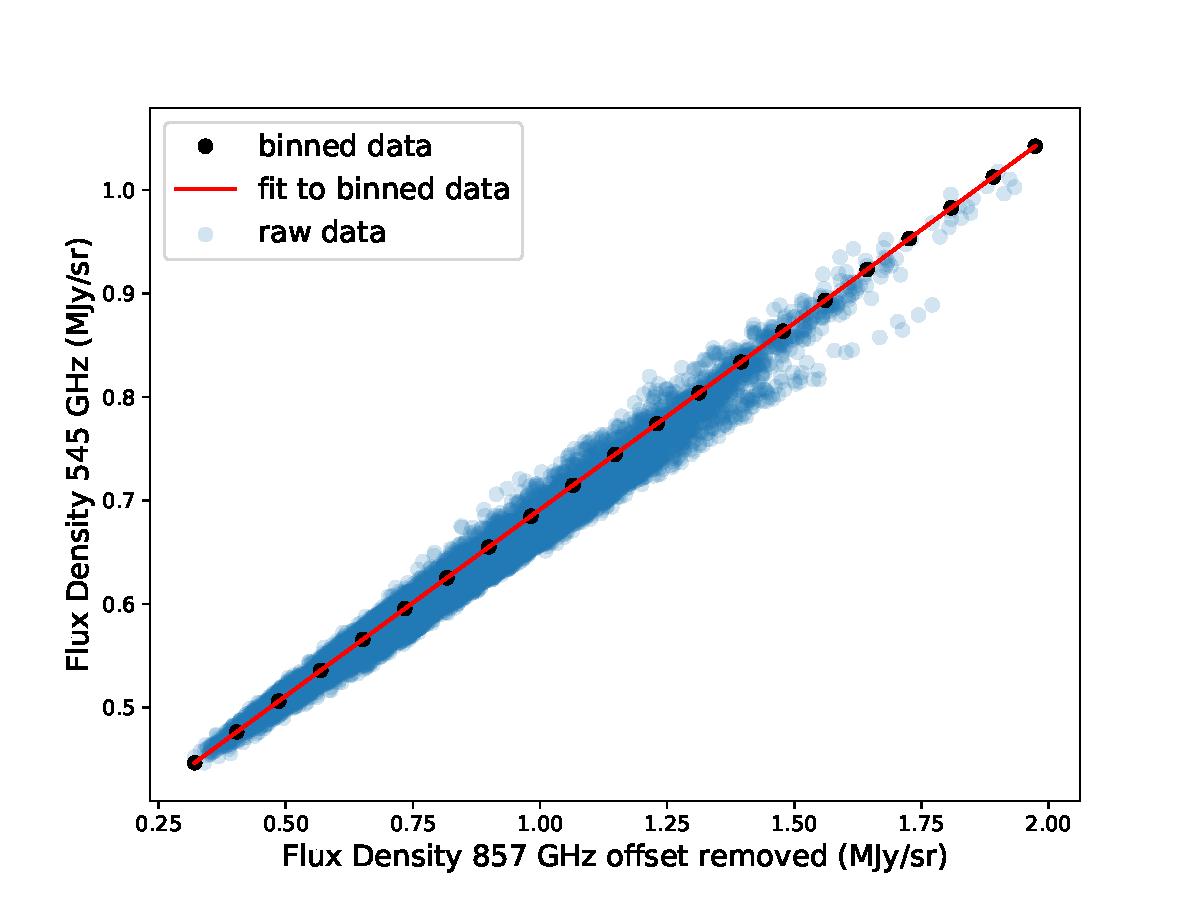
\includegraphics[width=0.8\linewidth]{ciboffsetEx}
\caption{An example of the linear regression used to determine the large scale CIB offset for each frequency.}
\label{fig:ciboffsetLinear}
\end{figure}

\section{GNILC methodology}\label{sec:apB}

The GNILC algorithm analysed in this work is based on that detailed in \citet{gnilc}. Our implementation is described here in full so that any differences may be highlighted. Instead of working on the sphere and using the needlet transform, the total flux maps were divided into twelve 2048X2048 pixel faces and the wavelet transform was used on the 2D faces. The optimum number of wavelet scales data was empirically found to be six, instead of the ten scales used by \citet{gnilc}. This difference can be explained by the fact that \citet{gnilc} work on all 12X2048X2048 pixels at once and the number of wavelet scales required is proportional to the log of the number of data samples. 

The following steps were completed for each wavelet scale ($j$). 
\begin{enumerate}[label*=\arabic*, nolistsep]
 \item The total flux maps were smoothed within the wavelet domain via convolution with a Gaussian of FWHM $2^{j} \times \frac{16\, \rm{pixels}}{2 \sqrt{2 \log{2}}}$. This width may be different from that used by \citet{gnilc}.  
 \item The nuisance terms were collected as N = CIB + CMB + instrumental noise. The $\rm{N_{obs}}$ by $\rm{N_{obs}}$ nuisance covariance matrix was calculated as:
\begin{equation}
{\bf{R}}_{{\rm{nus}}} = \frac{1}{\rm{npix}} \left({\bf{N \times N^{T} }} \right),  
\end{equation}     
 \item The covariance matrices of the smoothed total flux maps were calculated as $X_{a} \times X_{b}^{T} $, $X_{a/b}$ being the total flux within the wavelet domain at frequency $a/b$.
\item The $\rm{N_{obs}}$ by $\rm{N_{obs}}$ total flux covariance matrices for each smoothed pixel were whitened: ${\bf{R}}_{{\rm{nus}}}^{-1/2} {\bf{R}}_{{\rm{tot}}} {\bf{R}}_{{\rm{nus}}}^{-1/2}$.
\item The eigenvectors of each whitened covariance matrix were ordered and the Akaike Information Criterion was used to select eigenvalues which deviated significantly from unity. Those eigenvectors (${\bf{U}}_{s}$) gave the mixing matrix (${\bf{F}} = {\bf{R}}_{{\rm{nus}}}^{1/2} {\bf{U}}_{s} $) used to obtain the leat-squares optimisation of thermal dust emission ${\bf{F}} \left( {\bf{F}}^{T} {\bf{R}}_{{\rm{tot}}}^{-1} {\bf{F}} \right) {\bf{F}}^{T} {\bf{R}}_{{\rm{tot}}}^{-1} {\bf{X}}$ 
\item If no eigenvectors were identified as significant then the total flux was believed to be dominated by the nuisance terms and so the signal contribution at that pixel and wavelet scale was masked out (set to zero). 
\end{enumerate}
The thermal dust contributions at each wavelet scale were recomposed to form the GNILC estimate of thermal dust emission for each frequency within pixel space. 

%%%%%%%%%%%%%%%%%%%%%%%%%%%%%%%%%%%%%%%%%%%%%%%%%%


% Don't change these lines
\bsp	% typesetting comment
\label{lastpage}
\end{document}

% End of mnras_template.tex